\documentclass[12pt,letterpaper,noanswers]{exam}
\usepackage[usenames,dvipsnames,svgnames,table]{xcolor}
\usepackage[margin=0.9in]{geometry}
\renewcommand{\familydefault}{\sfdefault}
\usepackage{multicol}
\usepackage{wrapfig}
\pagestyle{head}
\definecolor{c03}{HTML}{FFDDDD}
\header{AM 22b Class 13}{}{Feb 26: cylindrical and spherical}
\runningheadrule
\headrule
\usepackage{graphicx} % more modern
\usepackage{amsmath} 
\usepackage{amssymb} 
\usepackage{hyperref}
\usepackage{tcolorbox}

\usepackage[numbered,autolinebreaks,useliterate]{mcode}

\newcommand{\mb}[1]{\underline{#1}}

\begin{document}
 \pdfpageheight 11in 
  \pdfpagewidth 8.5in




% I need to review the torus trajectories...

\begin{itemize}
% \item There is a pre-class assignment (20 minutes of videos + a few WeBWorK exercises) due at 10am this Monday.  It is available on Canvas.
\itemsep0em
    % \item PSet 02 is due on Friday Feb 14th at 10am.
   % \item There is a pre-class assignment due Monday by 10am (pre-class 03).
    \item Problem set 04 is due on Thursday Mar 4th at 6pm.
    \item Quiz 02 will be available Friday Mar 5th to Sunday Mar 7th at 6pm ET.
    \item There is a wellness day on Monday: no class or office hours.  Sarah's OH will be Wed 4-5pm and Thursday 2-3pm next week.
\end{itemize}

\hrule
\vspace{0.2cm}

% partial derivatives, gradient
% local linearity, differential, directional deriv
% 2nd order partials + equations with partials

\noindent\textbf{Big picture}

This week we are studying integration for functions of multiple variables.  Today our focus is on examples of changes of coordinates.

\vspace{0.2cm}
\hrule
\vspace{0.2cm}
\noindent\textbf{Skill Check C13 Practice}

\begin{questions}
\item (cylindrical coordinates) Sketch the region in $rz$-space associated with the region of integration in the integral below and describe the shape of the region.
\[\int_0^{2\pi}\int_0^{1/\sqrt{2}}\int_0^z rz\ dr\ dz\ d\theta.\]
\end{questions}

\vspace{0.2cm}
\hrule
\vspace{0.2cm}

\noindent\textbf{Skill Check C13 Solution}


\begin{lstlisting}
syms r z
fimplicit(@(r,z) r)
hold on
fimplicit(@(r,z) r-z)
fimplicit(@(r,z) z)
fimplicit(@(r,z) z-1/sqrt(2))
axis equal
fill([0, 0,1/sqrt(2)],[0,1/sqrt(2),1/sqrt(2)],'r')
xlabel('r'); ylabel('z');
axis([0 1 -0.2 1])
\end{lstlisting}

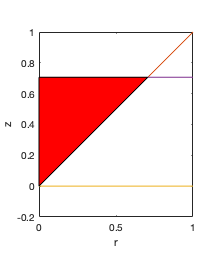
\includegraphics[scale=0.8]{img/C13skill.png}

The region is a solid cone.  (Imagine spinning this triangle around the $z$-axis through the angles $0$ to $2\pi$ to form the solid region).


\vspace{0.2cm}
\hrule
\vspace{0.2cm}

\eject

\noindent\textbf{Teams}
You will work with this team on the in-class problems today.  Introduce yourself to your team!
\begin{multicols}{2}
1.  students here

\end{multicols}

%\vspace{0.2cm}
\hrule
\vspace{0.2cm}

\noindent\textbf{Polar coordinates} \S 16.4

\begin{tcolorbox}

\begin{itemize}
\itemsep0em
    \item In polar coordinates, $x = r\cos\theta, y = r\sin\theta$.  $x^2+y^2 = r$.  
    \item The approximate area of a polar gridbox, $\Delta A$, is $\Delta A = (r\Delta\theta)\Delta r$, where $r\Delta\theta$ is the length of the circular arc and $\Delta r$ is the length of the radial segment.
    \item $\int_R f(x,y)\ dx\ dy = \int_R f(r\cos\theta,r\sin\theta)\ r\ dr\ d\theta$.
    \end{itemize}
    \end{tcolorbox}
    \begin{tcolorbox}

\begin{itemize}
\itemsep0em
    
    \item The conversion between $dxdy$ and $rdrd\theta$ can be found via the derivative (Jacobian) for the change of coordinates: Let $\underline x = \left(\begin{array}{c} x \\ y \end{array}\right)$ and $\underline u = \left(\begin{array}{c} r \\ \theta \end{array}\right)$.  We have $\dfrac{\partial \underline x}{\partial \underline u} = \left(\begin{array}{c c} \cos\theta & -r\sin\theta \\ \sin\theta & r\cos\theta \end{array}\right)$.  
    \item It turns out that $dA = 
    \left\vert\dfrac{\partial \underline x}{\partial \underline u}\right\vert d\overline{A}$ where $dA = dxdy$ and $d\overline{A} = drd\theta$.  $\dfrac{\partial \underline x}{\partial \underline u}$ is a linear transformation, and under the action of this transformation, a small box in $r,\theta$-space of area $d\overline{A}$ is transformed to a small box in $x,y$-space of area $dA = \left\vert\dfrac{\partial \underline x}{\partial \underline u}\right\vert d\overline{A}$.
\end{itemize}
\end{tcolorbox}


\noindent\textbf{Example (insect population).}  
The approximate population density of insects around a lake is estimated (in millions of insects per square kilometer) as shown in the figure below.  
\begin{itemize}
\itemsep0em
    \item The lake has a 2 km radius, and the outer circle has a 4 km radius.
\item Approximate the boxes as rectangles.  
\item The length of an arc of a circle is given by $r\Delta\theta$ where $r$ is the radius and $\Delta\Theta$ is the subtended angle.
\item Use a Riemann sum to estimate the total insect population that is within 1 km of the lake. 
\end{itemize}

 




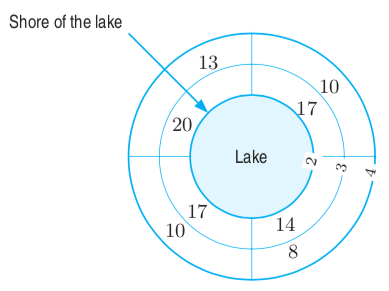
\includegraphics[width=2.5in]{img/C19p2.png}



\vspace{1in}

\noindent\textbf{Example: converting to polar}

Let $I = \displaystyle\int_{-\sqrt{\pi}}^{\sqrt{\pi}}\int_0^{\sqrt{\pi-y^2}}\sin(x^2+y^2)dx dy$.

To convert an integral from Cartesian to polar there are three steps:
\begin{enumerate}
    \item Convert the integrand: $\sin(x^2+y^2) = \sin(r^2)$.
    \item Convert $dA$:  $dxdy = rdrd\theta$.
    \item Convert the bounds:  Do this by converting the equations and sketching the region of integration.
    
    \begin{tabular}{| c c |}
        \hline
    $x = 0$ & $r\cos\theta = 0$ so $r = 0$ (not the case) or $\cos\theta = 0$, so $\theta = \pi/2$ or $\theta = -\pi/2$.\\
    \hline
    $x = \sqrt{\pi-y^2}$ & $\left\{\begin{array}{c} x^2+y^2 = \pi \\ x>0 \end{array}\right.$ so $\left\{\begin{array}{c}r^2 = \pi \\ -\pi/2<\theta<\pi/2\end{array}\right.$.  Simplifying,  $\left\{\begin{array}{c}r = \sqrt{\pi} \\ -\pi/2<\theta<\pi/2\end{array}\right.$\\
        \hline
    $y = -\sqrt{\pi}$ & $r\sin\theta = -\sqrt{\pi}$ \\
        \hline
    $y = \sqrt{\pi}$ & $r\sin\theta = \sqrt{\pi}$ \\
        \hline
    \end{tabular}
\end{enumerate}

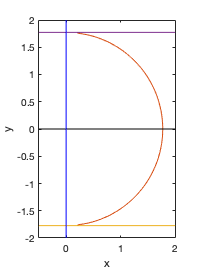
\includegraphics[height=2in]{img/C12-2dpolar.png}


\noindent\textbf{Example (function of integration).}  Identify the function of integration for the integral $\displaystyle\int_0^{\pi/4}\int_0^1r^2\cos\theta\ dr\ d\theta.$
  %\emph{pollQ}

% \instruct{Is it $r^2\cos\theta$ or $r\cos\theta$? Requires remembering $dA$ for polar...}

\vfill

\eject 
\noindent\textbf{Example (cartesian equivalent).}  Let $R$ be the region bounded by $x = 1$, $y=0$, $y=x$.  In polar coordinates, are the following integrals equal? \[\int_R x\ dA = \int_0^{\pi/4}\int_0^1r^2\cos\theta\ dr\ d\theta\]

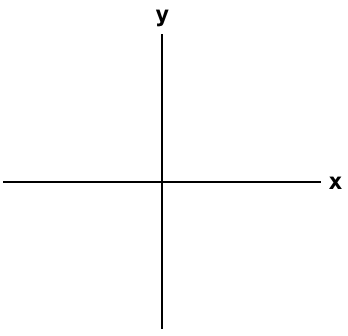
\includegraphics[height=2in]{img/C02axes-2.png}

%  \emph{pollQ}

%\instruct{yes+confident/not or no+confident/not.  A common mistake is to not notice the curved boundary for $R$ in the polar version.}

%\vfill



\noindent\textbf{Example (change coordinates)}.  Rewrite $\displaystyle \int_0^{\pi/4}\int_0^1r^2\cos\theta\ dr\ d\theta$ in Cartesian coordinates.  %Use horizontal stripes.

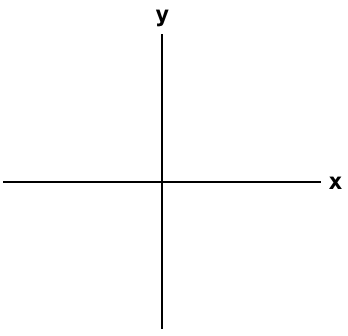
\includegraphics[height=2in]{img/C02axes-2.png}

% \instruct{incorporate terms horizontally simple and vertically simple}
%\vfill

\eject
\noindent\textbf{Region of integration vocabulary}
\begin{tcolorbox}
\begin{itemize}
\itemsep0em
    \item A region of integration is called \textbf{horizontally simple} the region $R$ is of the form 
$c\leq y\leq d$, 
$h_1(y)\leq x \leq h_2(y)$, so 
$\int_R f\ dA = \int_c^d\int_{h_1(y)}^{h_2(y)} f\  dx\ dy$ 
(the integral can be written using a single iterated integral using horizontal stripes).
\item A region of integration is called \textbf{vertically simple} the region $R$ is of the form $c\leq x\leq d$, $h_1(x)\leq y \leq h_2(x)$, so $\int_R f\ dA = \int_c^d\int_{h_1(x)}^{h_2(x)} f\ dy\ dx$ (the integral can be written using a single iterated integral using vertical stripes).
\end{itemize}

\end{tcolorbox}
%\eject

\vspace{0.2cm}
\hrule
\vspace{0.2cm}

\noindent\textbf{Cylindrical coordinates} \S 16.5
\begin{tcolorbox}
\begin{itemize}
\itemsep0em
    \item  In the \textbf{cylindrical coordinate} system, each point in $3$-space is represented using $0\leq r < \infty, 0\leq \theta\leq 2\pi, -\infty < z < \infty.$  $x = r\cos\theta, y = r\sin\theta, z = z.$  Note that $x^2+y^2 = r^2.$
    \item A region $a\leq r\leq b, c\leq \theta\leq d, m\leq z \leq n$, where all bounds are constants, will be a piece of a solid circular cylinder.
    \end{itemize}
    \end{tcolorbox}
    
    \noindent\textbf{Example (cylindrical coordinates).} 

The region shown in D is the region where $1\leq r \leq 2,$  $\pi/8\leq \theta\leq \pi/4,$ and $ 1\leq z \leq 3.$

Match plots A, B, C to the following pairs of surfaces
\begin{itemize}
\item
$r = 1,$ $\pi/8\leq \theta\leq \pi/4,$ $ 1\leq z \leq 3$ and  $r = 2,$ $\pi/8\leq \theta\leq \pi/4,$ $ 1\leq z \leq 3.$
\item $1\leq r \leq 2,$ $\theta = \pi/8,$ $ 1\leq z \leq 3$ and  $1\leq r \leq 2,$ $ \theta =  \pi/4,$ $ 1\leq z \leq 3.$
\item $1\leq r \leq 2$, $\pi/8\leq \theta\leq \pi/4,$ $ z = 1$ and  $1\leq r \leq 2,$ $\pi/8\leq \theta\leq \pi/4,$ $z = 3.$  %\emph{pollQ}
\end{itemize}

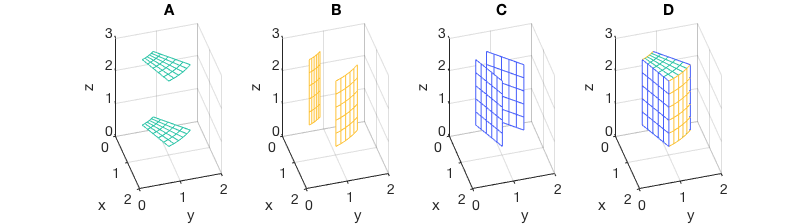
\includegraphics[width=\linewidth]{img/C20p1.png}
    
    \eject
    
    \noindent\textbf{Integration using cylindrical coordinates} \S 16.5
    \begin{tcolorbox}
    \begin{itemize}
    \item $\displaystyle\left\vert \frac{\partial(x,y)}{\partial(r,\theta)}\right\vert$ is called the \textbf{Jacobian determinant} or sometimes the \textbf{Jacobian} for the coordinate transformation from $(x,y)$ to $(r,\theta)$.
    \item $\displaystyle\left\vert \frac{\partial(x,y)}{\partial(r,\theta)}\right\vert = \left\vert\begin{array}{c c} \cos\theta & -r\sin\theta \\ \sin\theta & r\cos\theta \end{array}\right\vert = r\cos^2\theta + r\sin^2\theta = r$.  We have $dA = dxdy = \displaystyle\left\vert \frac{\partial(x,y)}{\partial(r,\theta)}\right\vert\ drd\theta = rdrd\theta$
    \item The \textbf{Jacobian} for the change of coordinates from Cartesian to cylindrical, $\displaystyle\left\vert\frac{\partial(x,y,z)}{\partial(r,\theta,z)}\right\vert$ is $r$.  The volume element is given by $dV = rdrd\theta dz = dxdydz$.
\end{itemize}


  %When $r$ changes by $\Delta r$, $x$ and $y$ change by approximately $\cos\theta \Delta r$ and $\sin\theta\Delta r$, respectively.  When $\theta$ changes by $\Delta \theta$, $x$ and $y$ change by approximately $-r\sin\theta\Delta\theta$ and $r\cos\theta\Delt$
\end{tcolorbox}





\noindent\textbf{Region of integration in cylindrical coordinates} \S 16.5
\begin{tcolorbox}
\begin{itemize}
\itemsep0em
    \item Given an integral, $\int_W f\ dV$, expressed in cylindrical coordinates, sketching a cross-section of the region of integration in  $rz$-space is an important step in identifying the region. 
\end{itemize}


  %When $r$ changes by $\Delta r$, $x$ and $y$ change by approximately $\cos\theta \Delta r$ and $\sin\theta\Delta r$, respectively.  When $\theta$ changes by $\Delta \theta$, $x$ and $y$ change by approximately $-r\sin\theta\Delta\theta$ and $r\cos\theta\Delt$
\end{tcolorbox}

\noindent\textbf{Example (cylindrical region).}  Consider a water tank, where the water has depth $h$.  Let the volume of water in the tank be given by \[\int_0^{2\pi}\int_0^h\int_0^{\sqrt{a^2-z^2}} r\ dr\ dz\ d\theta.\]
\begin{itemize}
    \item Identify the function of integration.
    \item Sketch a representative cross section of the region of integration in the $rz$-half plane.
    \item Describe the shape of the water tank.
\end{itemize} 

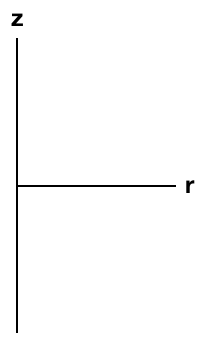
\includegraphics[height=2in]{img/C13rzaxes.png}



% \noindent\textbf{Example ($x = 2$ in cylindrical).}  How could we represent volume of the triangular box $1\leq x \leq 2$, $0\leq y\leq x$, $-1\leq z \leq 0$ in cylindrical coordinates?

% $x = 1$ becomes $r\cos\theta = 1$ so $r = \frac{1}{\cos\theta}$.  Similarly, $x = 2$ becomes $r = \frac{1}{\cos\theta}$.  \[\int_{-1}^0\int_0^{\pi/4}\int_{1/\cos\theta}^{2/\cos\theta}1\ r\ dr\ d\theta\ dz.\]

% \includegraphics[width=2in]{img/C20p4.png}

\vspace{0.2cm}
\hrule
\vspace{0.2cm}

\eject

\noindent\textbf{Spherical coordinates} \S 16.5
\begin{tcolorbox}
\begin{itemize}
\itemsep0em
    \item In the \textbf{spherical coordinate} system, each point in $3$-space is represented using $0\leq \rho < \infty, 0\leq \theta\leq 2\pi, 0 \leq \phi\leq \pi.$  
    \item The spherical coordinates are most easily understood in terms of cylindrical coordinates: $z = \rho\cos\phi,$ $r = \rho\sin\phi$.
    
    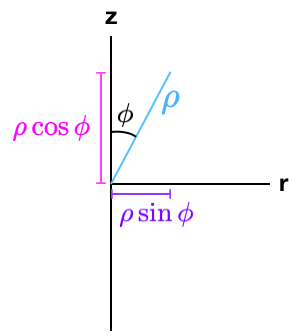
\includegraphics[width=1.7in]{img/C13spherical.png}
    
    \item Translating back to Cartesian: $x = r\cos\theta = \rho\sin\phi\cos\theta$ and $y = r\sin\theta = r\sin\phi\sin\theta$.  Note that $x^2+y^2 +z^2= \rho^2.$
    \item A region $a\leq \rho\leq b, c\leq \theta\leq d, m\leq \phi \leq n$, where all bounds are constants, will be a piece of a solid spherical ball.
    \end{itemize}
    \end{tcolorbox}
    
    \noindent\textbf{Example (spherical coordinates).}

The region shown in D is the region where $1\leq \rho \leq 2,$  $\pi/8\leq \theta\leq 3\pi/8,$ and $ \pi/4\leq \phi \leq 7\pi/6.$

Which of A, B, C is associated with the $\theta = c$ surfaces (for $c$ some constant)? 

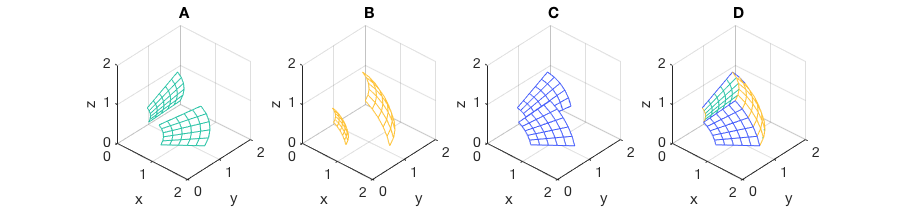
\includegraphics[width=\linewidth]{img/C20p5.png}



\noindent\textbf{Example ($\phi = c$).}

In plot $A$ below are shown two surfaces on which $\phi$ is held constant.  On which surface is $\phi$ greater? 

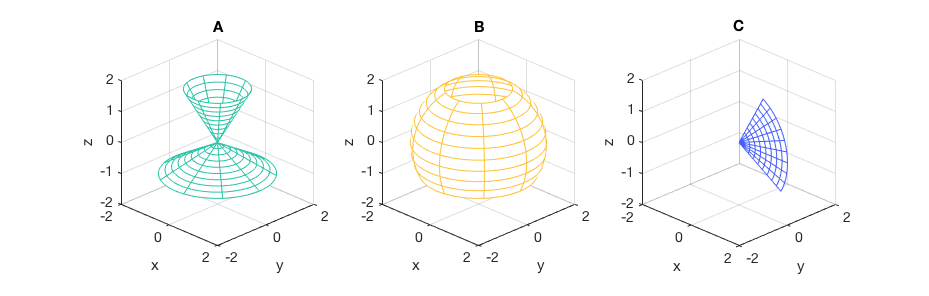
\includegraphics[width=0.8\linewidth]{img/C20p7.png}
    
    
    \eject
    \noindent\textbf{Integration using spherical coordinates} \S 16.5
    \begin{tcolorbox}
    \begin{itemize}
\item The \emph{Jacobian} for the change of coordinates from Cartesian to spherical, $\displaystyle\left\vert\frac{\partial(x,y,z)}{\partial(\rho,\theta,\phi)}\right\vert$, is $\rho^2\sin\phi$ so the volume element is given by $dV = \rho^2\sin\phi\ d\rho\ d\theta\ d\phi$.

\end{itemize} 




  %When $r$ changes by $\Delta r$, $x$ and $y$ change by approximately $\cos\theta \Delta r$ and $\sin\theta\Delta r$, respectively.  When $\theta$ changes by $\Delta \theta$, $x$ and $y$ change by approximately $-r\sin\theta\Delta\theta$ and $r\cos\theta\Delt$
\end{tcolorbox}


\noindent\textbf{Example}

A half-melon is approximated by the region between two spheres, one of radius $a$ and the other of radius $b$, with $0<a<b$.  Write a triple integral, including limits of integration, giving the volume of the half-melon.

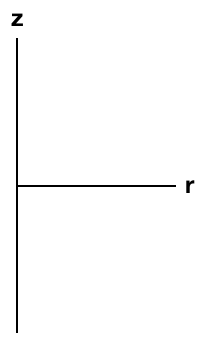
\includegraphics[height=2in]{img/C13rzaxes.png}

\noindent\textbf{Exercises}

Set up the following triple integrals using either cylindrical or spherical coordinates.  Start by sketching a cut through each region in the $rz$-half plane.
\begin{parts}
\item Triple integral to find the volume of the region $W$ that is inside the sphere of radius $5$ centered at the origin \textbf{and} inside the cylinder of radius $3$ centered about the $z$-axis.  \emph{This looks like a solid cylinder with spherical caps}.
\item Triple integral to find the volume of the region $W$ inside the sphere $x^2+y^2+z^2 = 2$ and outside the double cone $z^2=x^2+y^2$ ($W$ contains the portion of the $xy$-plane within the sphere).
\item Redo your setups above in the other coordinate system.
\end{parts}

\vfill


\eject


\noindent\textbf{Problem}


The figure below shows part of a spherical ball of radius $5$ cm.  Write an iterated triple integral which represents the volume of this region.

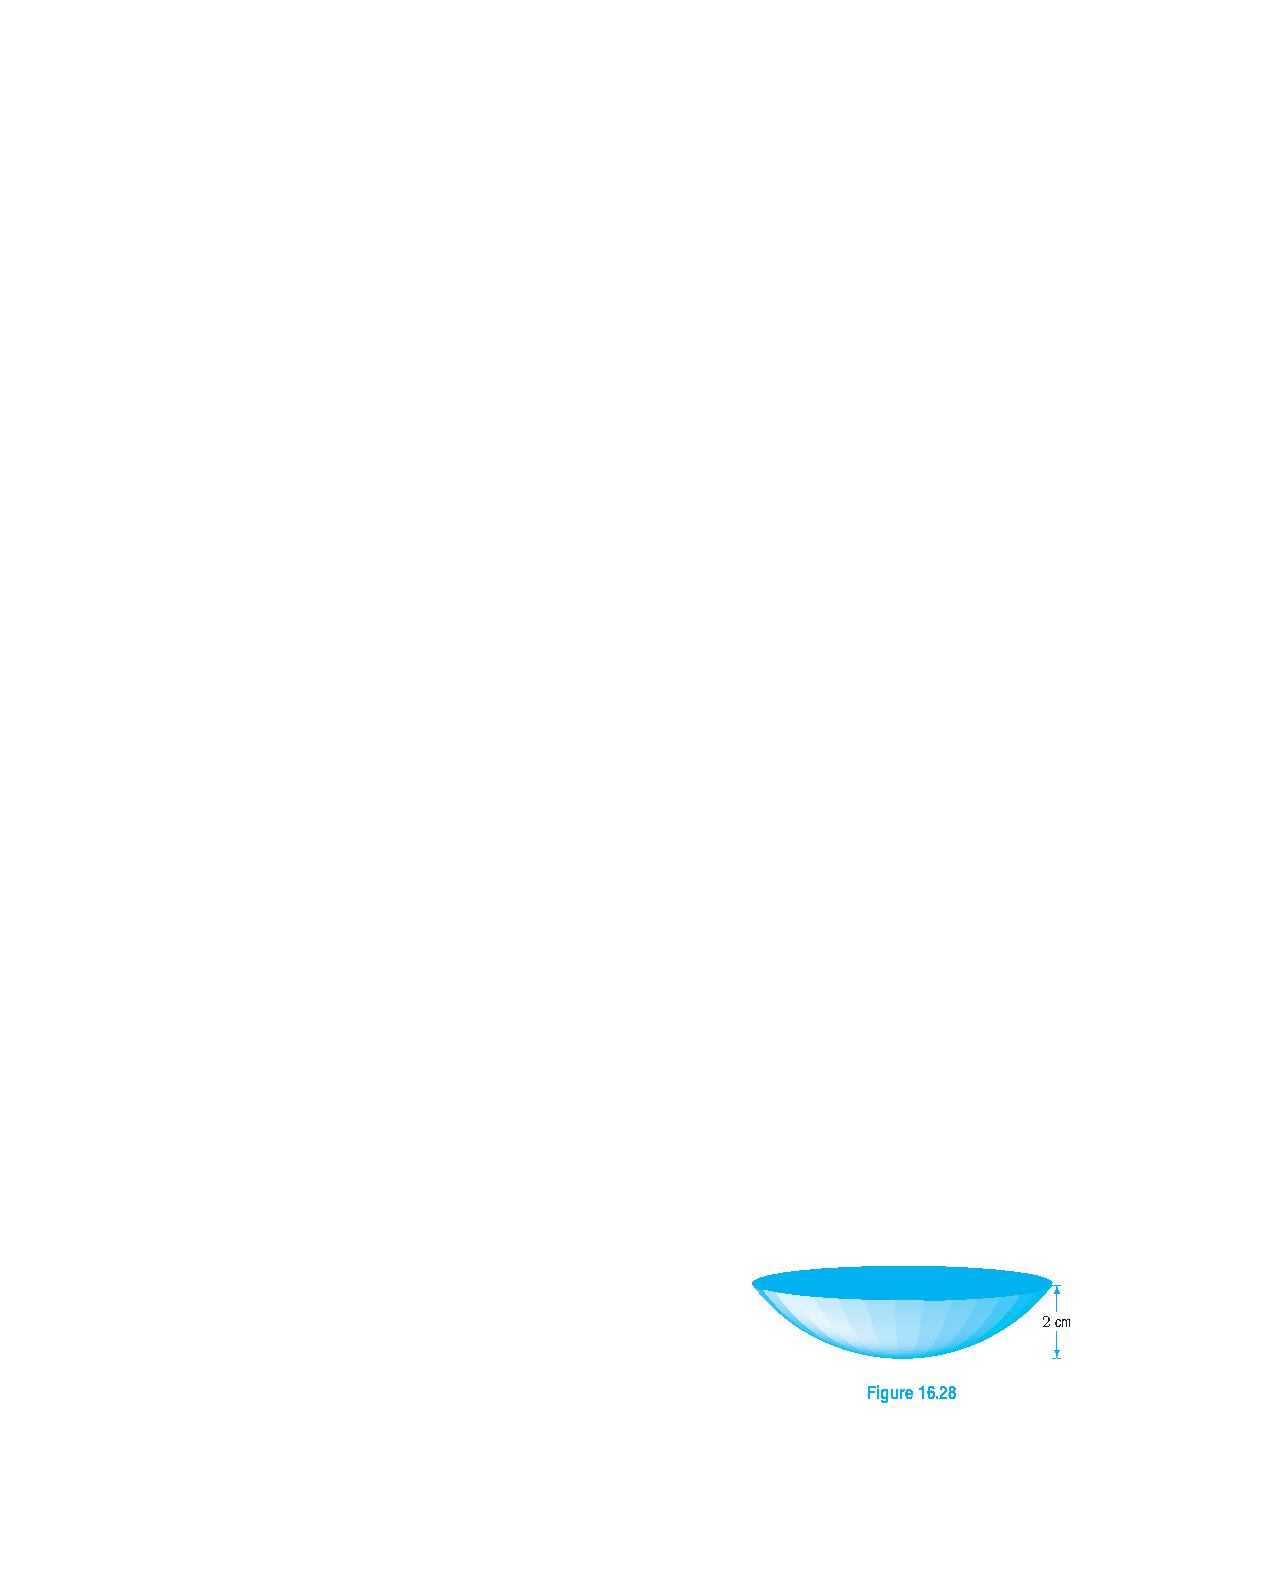
\includegraphics{img/W05p2.pdf}


%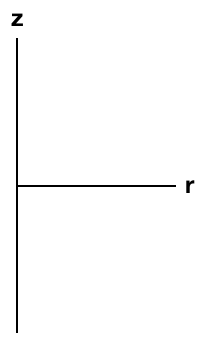
\includegraphics[height=2in]{img/C13rzaxes.png}
\vfill

Answers to exercises: $\int_0^{2\pi}\int_0^3\int_{-\sqrt{5-r^2}}^{\sqrt{5-r^2}}1\ r\ dz\ dr\ d\theta$.  $\int_0^{2\pi}\int_0^{\sqrt{2}}\int_{\pi/4}^{3\pi/4} \rho^2\sin\phi\ d\phi\ d\rho\ d\theta$.


\end{document}